\chapter{Genomic Location Effect}\label{gle}

The tendency for mutations to occur in closed \gls{chromatin} regions has been reported both in cancer and other mutagenesis processes \citep{Polak2015,Prendergast2007ChromatinGenome}. This is hypothetically because closed chromatin regions, despite being less exposed to mutagens, are harder for repair systems to reach \citep{Prendergast2007ChromatinGenome,Teng1997ExcisionSequences, Morse2002PhotoreactivationCerevisiae}. Section \ref{gle:chromatin} of this chapter shows further evidence that mutations did tend to occur in closed rather than open chromatin regions. However, despite its influence on \gls{gle}, chromatin structure was unlikely to determine whether GLE was discriminative of cancers or not. Nevertheless, section \ref{gle:bootstrap} shows that \gls{gle} was significantly different between cancers, irrespective of the driving mechanisms. 

\section{Mutation location was influenced by chromatin status}\label{gle:chromatin}
My analyses of GLE were motivated by observations sugesting mutations tend to locate in closed chromatin regions. Figure \ref{fig:mutation_density} shows the distribution of mutations on chromosome 12 for four cancers, the others are in the Appendix Figure \ref{fig:apdx_mutation_density}. The choice to display chromosome 12 was arbitrary, other chromosomes are available upon request. The shaded DHS bars near the bottom of the plots are hypersensitive regions (open chromatin) for the original cells, which was identified by literature search, shown in Table \ref{tab:encode}. By visualisation, it can already be seen that mutation density was greater in less dense DHS, indicating a bias towards closed chromatin regions for the cancers of interest. This pattern was particularly strong in Skin-Melanoma and Liver-HCC, and less obvious in Kidney-RCC. It is also worth noting that the chromatin structures appeared locally different between cancers but there were some globally common patterns across the chromosome. Looking at the density by itself, we could see a diversity in how mutations are distributed, supporting the potential of GLE in discriminating cancers. 

\begin{figure}[ht!]
    \begin{subfigure}{.5\textwidth}
    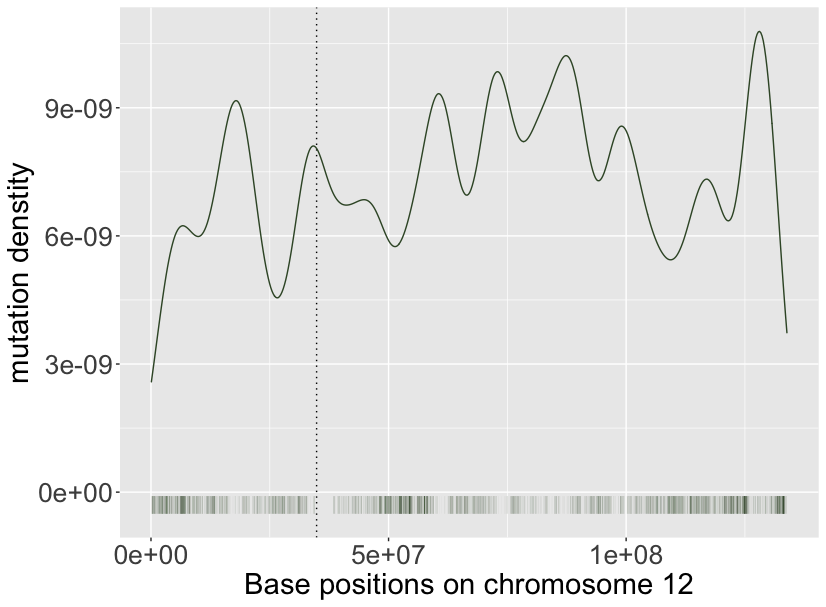
\includegraphics[width=\linewidth,height=0.7\textwidth]{graphics/mutdistribution_Skin-Melanoma.png}
    \caption{Skin-Melanoma}
    \label{fig:density_skin}
    \end{subfigure}
    ~
    \begin{subfigure}{.5\textwidth}
    
    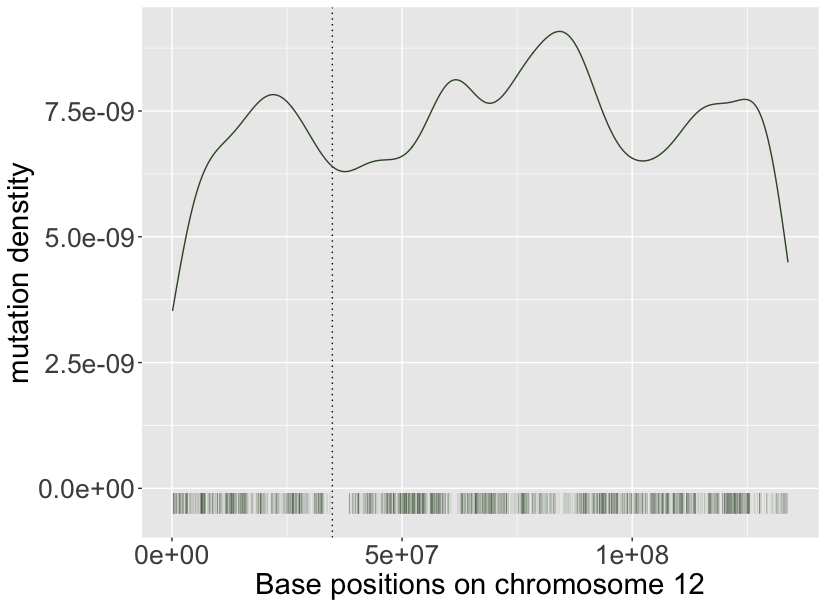
\includegraphics[width=\linewidth,height=0.7\textwidth]{graphics/mutdistribution_Kidney-RCC.png}
    \caption{Kidney-RCC}
    \label{fig:density_kidney}
    \end{subfigure} \\
    \vspace{0.5cm}
    
    \begin{subfigure}{.5\textwidth}
    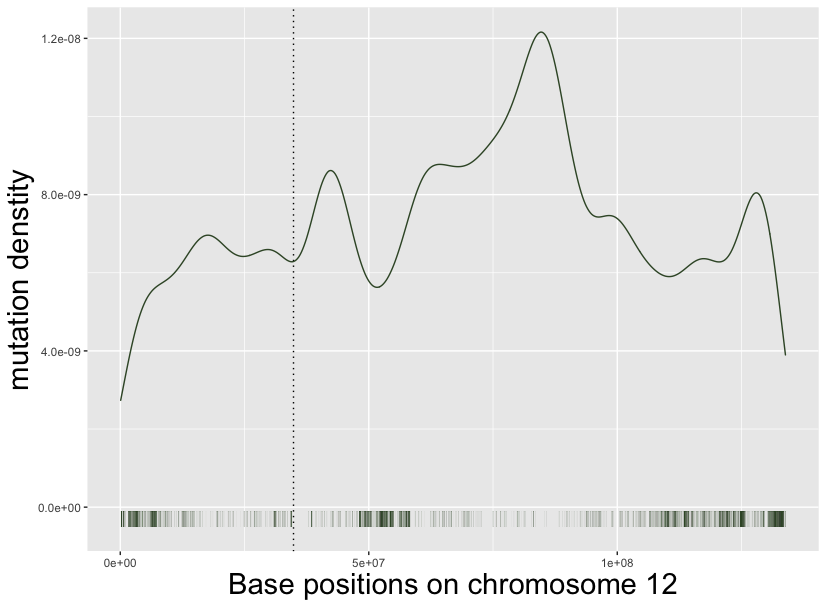
\includegraphics[width=\linewidth,height=0.7\textwidth]{graphics/mutdistribution_Liver-HCC.png}
    \caption{Liver-HCC}
    \label{fig:density_liver}
    \end{subfigure}
    ~
    \begin{subfigure}{.5\textwidth}
    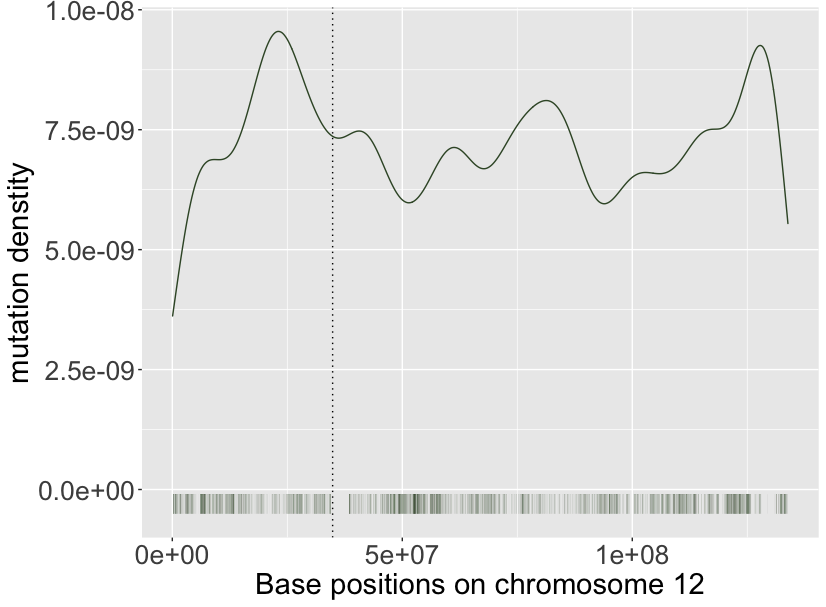
\includegraphics[width=\linewidth,height=0.7\textwidth]{graphics/mutdistribution_Panc-AdenoCA.png}
    \caption{Panc-AdenoCA}
    \label{fig:density_panc_adenoca}
    \end{subfigure} \\
    \caption{\textbf{Mutations tend to be found in closed chromatin regions.} Different cancers differ in the distribution of mutations across the genome. Here chromosome 12 is shown. (a) Skin-Melanoma (b) Kidney-RCC (c) Liver-HCC (d) Panc-AdenoCA, the other cancers are shown in Figure \ref{fig:apdx_mutation_density}. The shaded bars below the x-axis indicate open chromatin regions, the gaps indicate closed chromatin regions of the original cell types. The vertical dotted line indicates the position of the centromere.}
    \label{fig:mutation_density}
\end{figure}

\subsection{Some cancers were more similar than others in terms of chromatin structures}\label{gle:pca}
In investigating whether the diversity in GLE is influenced by chromatin structure, one factor worth considering is how cancers relate to each other by the chromatin structure of their original cells to begin with. To compute the difference between the DHS of two original cell types, I identified the span of the intersection of their open chromatin regions and converted it into a distance (Methods \ref{methods:encode_pca}). The distance between every pair of cells allows calculating and visualising their relative coordinates using multidimensional scaling. Figure \ref{fig:encode_pca} shows the three most informative dimensions (PC1, PC2 and PC3; in descending order of informativeness) for the relationship between the cells of origin. Melanocyte and hepatocyte had the most distinct chromatin structures as they were relatively far away from the other cell types. On the other hand, prostate epithelium (ProstEpi) and exocrine cells of the pancreatic duct (PancDuct) were very close with respect to DHS on both panels.

% \begin{figure}[h!]
%     \begin{subfigure}{.5\textwidth}
%     \centering
%     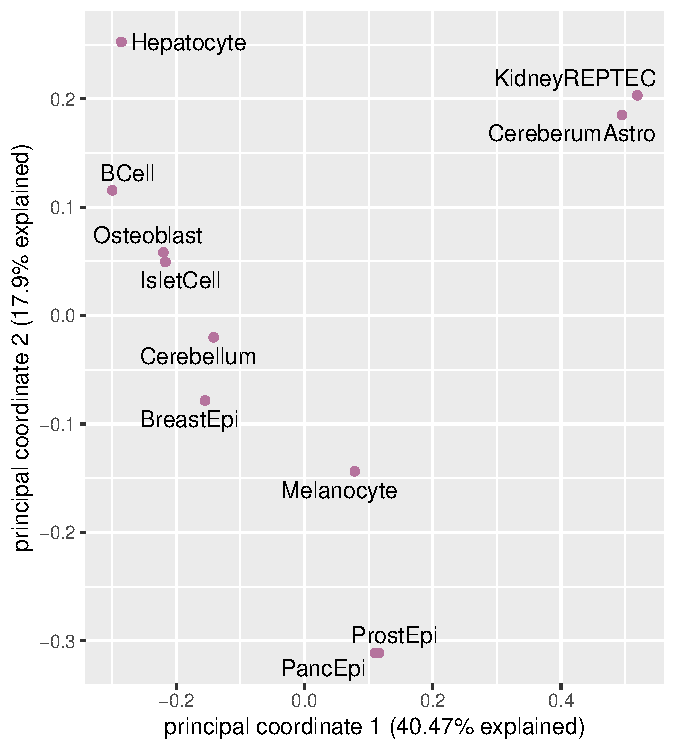
\includegraphics[scale=0.7]{graphics/encode_pca_1_2.pdf}
%     \caption{PC2 \textit{v.s.} PC1}
%     \end{subfigure}
%     ~
%     \begin{subfigure}{.5\textwidth}
%     \centering
%     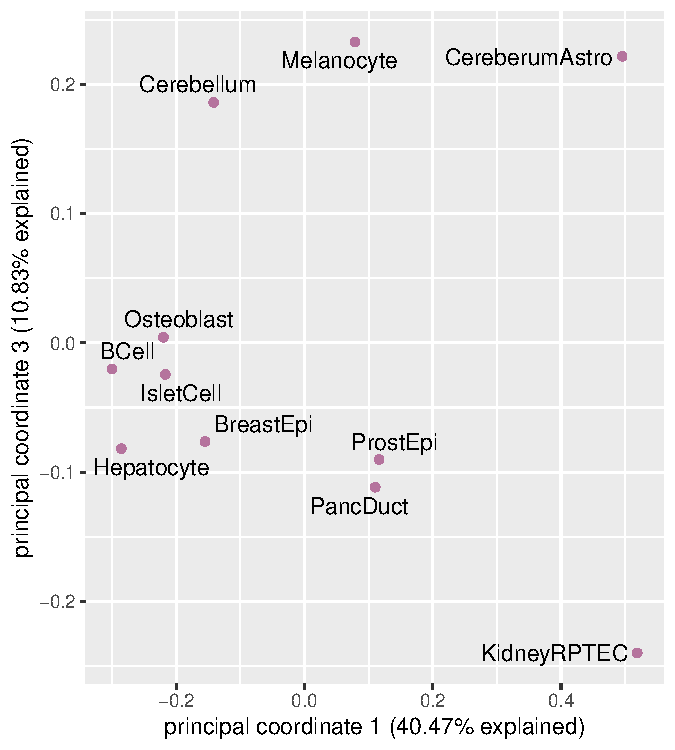
\includegraphics[scale=0.7]{graphics/encode_pca_1_3.pdf}
%     \caption{PC3 \textit{v.s.} PC1}
%     \end{subfigure} \\
%     \caption{\textbf{PCA}.}
%     \label{fig:encode_pca}
% \end{figure}

\begin{figure}[h!]
  \begin{minipage}[c]{\textwidth}
    \begin{subfigure}{.5\textwidth}
    \centering
    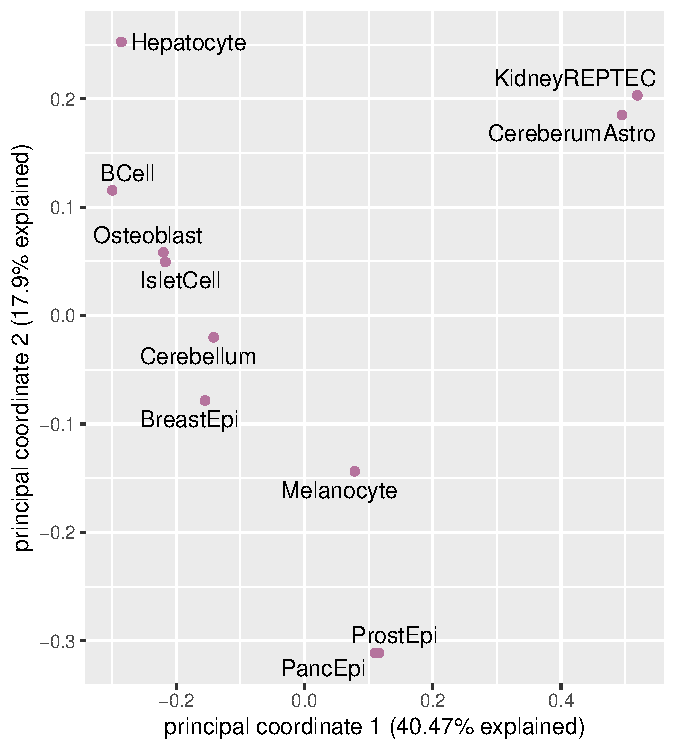
\includegraphics[scale=0.7]{graphics/encode_pca_1_2.pdf}
    \caption{PC2 \textit{v.s.} PC1}
    \end{subfigure}
    ~
    \begin{subfigure}{.5\textwidth}
    \centering
    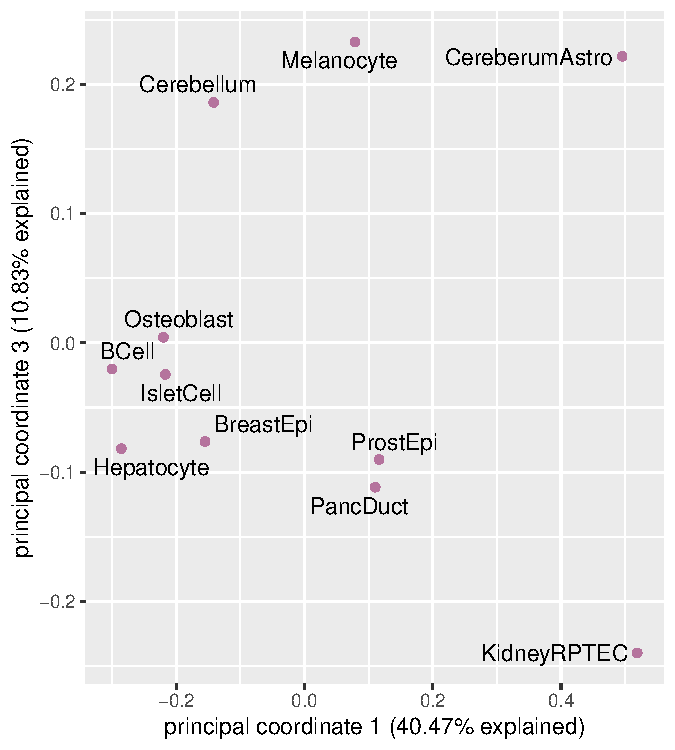
\includegraphics[scale=0.7]{graphics/encode_pca_1_3.pdf}
    \caption{PC3 \textit{v.s.} PC1}
    \end{subfigure} \\
  \end{minipage}\hfill
  \vspace{1cm}
  
  \begin{minipage}[c]{\textwidth}
    \centering
    \begin{tabulary}{\textwidth}{ ll }
    \toprule
    \textbf{Original cell abbreviation} & \bf{Cancer Type}  \\
    \toprule
    Osteoblast & Osteosarcoma \\
    
    BreastEpi & Breast-AdenoCa \\
    
    Cerebellum &  CNS-Medullo  \\
    
    CereberumAstro & CNS-PiloAstro \\
    
    KidneyRPTEC & Kidney-RCC \\
    
    Hepatocyte & Liver-HCC \\
    
    BCell & Lymph-BNHL, Lymph-CLL \\
    
    PancDuct & Panc-AdenoCa \\
    
    IsletCell & Panc-Endocrine \\
    
    ProstEpi & Prost-AdenoCa \\
    
    Melanocyte & Skin-Melanoma \\
    \bottomrule
    
    \end{tabulary}
    
    % . DHS data for these cells is downloaded from either \href{https://genome.ucsc.edu/cgi-bin/hgFileUi?db=hg19&g=wgEncodeOpenChromDnase}{Duke} or \href{https://genome.ucsc.edu/cgi-bin/hgFileUi?db=hg19&g=wgEncodeUwDnase}{UW} project
  \end{minipage}\hfill
  \vspace{0.5cm}
  
  \begin{minipage}[c]{\textwidth}
    \caption{
      \textbf{Some cancers were more related in terms of chromatin structures than others.} Here, I visualised the relative coordinates of the original cell types for cancers on the most informative dimensions (principle coordinates, PC). This was done by multidimensional scaling of the pairwise distance between cell types. The distance between two cell types was computed based on the intersection between their open chromatin regions. 
    } \label{fig:encode_pca}
  \end{minipage}
\end{figure}


\subsection{Open and closed chromatin regions have significantly different mutation rates}\label{gle:g}
Having visualised the tendency of mutation location and the relationship between the chromatin structures of the original cells, I performed a hypothesis test to confirm whether there was a difference in how mutations are distributed between open and closed chromatin regions. This was achieved using the G-test of independence (Methods \ref{methods:chromatin}). The p-values obtained from this were adjusted using Bonferroni multiple test correction (Table \ref{tab:g-test}, the raw counts are in Appendix \ref{apdx:g-test}). To begin with, the size of the regions identified as open chromatin was considerably tiny compared to that of closed chromatin regions. Keeping that in mind, we can see that most cancers had significantly different mutation rates between open and closed chromatin regions, except CNS-PiloAstro and Panc-Endocrine. Note that these two cancers had small to modest numbers of mutations. While no direct correlation between p-values and number of mutations could be detected, no cancers with less than 1 million mutations gave a p-value $>10^{-100}$. While this implied the impact of the number of mutations on the power of the test, our conclusion remains that mutation location was not random between open and closed chromatin regions. 

% latex table generated in R 4.1.0 by xtable 1.8-4 package
% Tue Oct 19 08:53:20 2021
\begin{table}[h]
\centering
\caption{\textbf{The chance of mutations occurring are significantly different between closed and open regions for most cancers.} The table presents }
\label{tab:g-test}
\begin{tabular}{lrr}
  \toprule
 \textbf{Disease} & \textbf{$\hat{p}$-value} & \textbf{Number of mutations} \\ 
  \hline
 Bone-Osteosarc & 5.66 $\times 10^{-35}$ & 166845 \\ 
 Breast-AdenoCa & 1.33 $\times 10^{-10}$ & 713855 \\ 
 CNS-Medullo & 2.46 $\times 10^{-34}$ & 209997 \\ 
 CNS-PiloAstro & 1.00 & 22020 \\ 
 Kidney-RCC & 2.60 $\times 10^{-06}$ & 531886 \\ 
 Liver-HCC & $<10^{-100}$ & 3321521 \\ 
 Lymph-BNHL & $<10^{-100}$ & 1124881 \\ 
 Lymph-CLL & $<10^{-100}$ & 226242 \\ 
 Panc-AdenoCA & $<10^{-100}$ & 1675781 \\ 
 Panc-Endocrine & 8.82 $\times 10^{-02}$ & 258564 \\ 
 Prost-AdenoCA & 5.49 $\times 10^{-90}$ & 1000496 \\ 
 Skin-Melanoma & $<10^{-100}$ & 7770980 \\ 
   \bottomrule
\end{tabular}
\end{table}

\subsection{Mutations were typically biased towards closed regions}\label{gle:or}
Complementary to the G-tests, which suggested that the difference in mutation location were statistically significance between closed and open chromatin regions, I computed the odds ratio ($OR$), which measures the direction of this difference. From equation \ref{eq:or} (Methods \ref{methods:chromatin}), $OR$ compares the ratios of mutated over non-mutated positions between closed and open chromatin regions. An $OR>1$ indicates a bias towards closed regions, and an $OR<1$ indicates a bias towards open regions. For each cancer, I estimated the standard error of $OR$'s using jackknife, where one donor was removed to obtain a pseudo-value for $OR$. The standard errors of the resulting sample of $OR^{pseudo}$ were the jackknifed standard error for $OR$. The results are shown in Figure \ref{fig:or_jackknifed}.

\begin{figure}[h!]
    \centering
    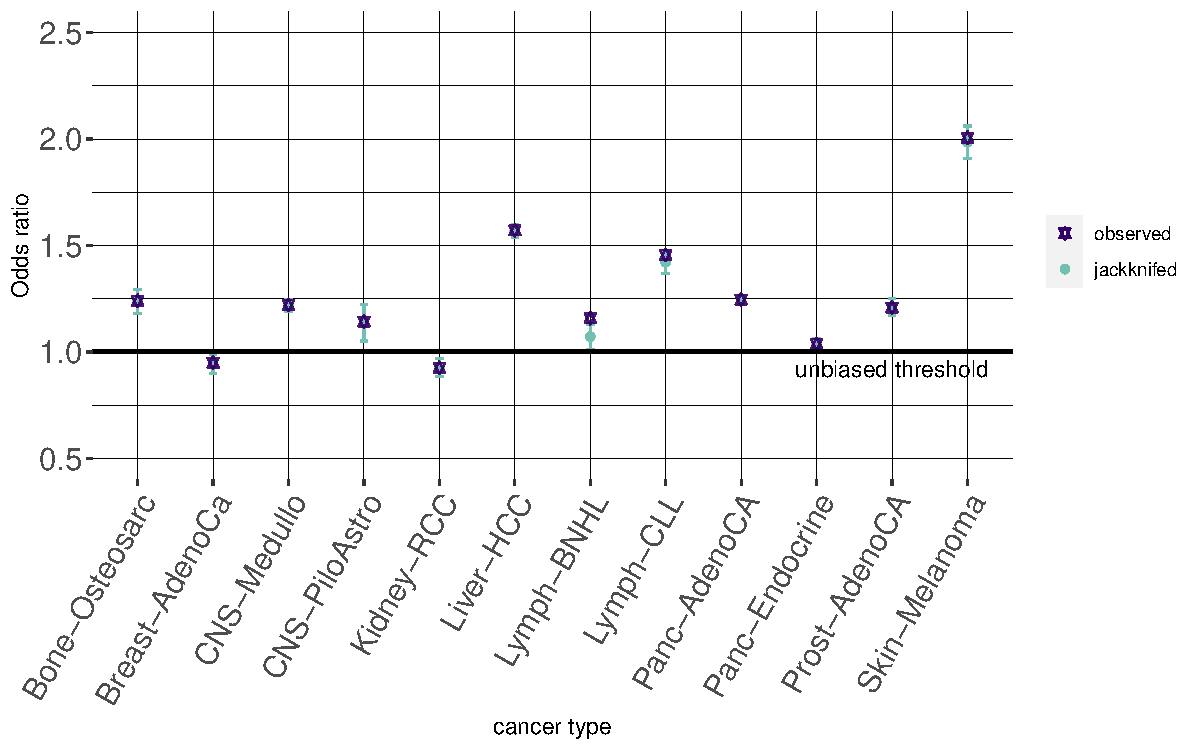
\includegraphics[scale=0.8]{graphics/jackknife_OR.pdf}
    \caption{\textbf{Mutations tend to occur in closed chromatin regions according to the odds ratio ($OR$) statistic}. $OR>1$ indicates a bias towards towards closed regions, and $OR<1$ indicates the opposite. Error bars are the standard errors of the jackknifed sample. The green circles are the means of the jackknifed pseudo-values. The purple stars are the observed $OR$.}
    \label{fig:or_jackknifed}
\end{figure}


Overall, mutations preferred to locate in closed chromatin regions, especially for Skin-Melanoma ($OR=2$). However, this bias varied between cancers. In addition, there are three other intriguing features. First, Breast-AdenoCa and Kidney-RCC had $OR<1$. Their p-values from the G-test showed a significant difference between closed and open regions, suggesting that the observed preference for open regions was not due to noise. On the density plots (Figures \ref{fig:mutation_density} and \ref{fig:apdx_mutation_density}), mutations still peaked at closed chromatin regions, but less clear than for example Skin-Melanoma. Second, the departure of the observed $OR$ from the mean pseudo-values in Lymph-BNHL and Lymph-CLL suggests an abnormality in these cases. This abnormality could be due to the large variance of GLE in donors with these cancers. However, it could also come from the uncertainty in identifying the original cells (one DHS sample of B cells for both Lymph-BNHL and Lymph-CLL, discussed in Section \ref{discussion:gle}). Third, CNS-PiloAstro had the largest standard error of $OR$. Again, this might be because its small number of mutations lowered the signal to noise ratio compared to other cancers, which is consistent with the G-test results. Regarding reliability, empirically, $OR$ seemed more robust to the number of mutations than G-test. Mathematically, it accounts for the imbalance in the size of open \textit{v.s.} closed chromatin regions. However, we need to be vigilant about the existence of this imbalance.

\subsection{Chromatin structure was influential but not discriminative}\label{gle:mixed_or}

In this subsection, I evaluated the appropriateness of $OR$ given the imbalance between the size of open and closed chromatin regions and the potential of $OR$ in discriminating cancers. The evaluation was done by calculating the $OR$'s with mislabelled DHS data. That is, mislabelled $OR$ was calculated by sorting a cancer's mutation data based on other cancers' DHS data rather than its own (Methods \ref{methods:chromatin}). 

The impact of imbalanced DHS was assessed in Figure \ref{fig:mixed_or_violin}. Specifically, I examined whether the very large size of closed chromatin regions rather than its biological properties made mutations in closed regions more likely than in open regions. If $OR$ was sensitive to the imbalance, each violin should have had a distinctive value. A good example to illustrate this involves Skin-Melanoma and Kidney-RCC, whose ratios of closed over open chromatin regions were 65:1 and 115:1 in their original cells' DHS, respectively (Table \ref{fig:tab_g-test_contingency}). If $OR$ was sensitive, it should have always been higher in Kidney-RCC than Skin-Melanoma, no matter what mutation data was used. This was not the case. $OR$ range was approximately the same for Kidney-RCC and Skin-Melanoma, which suggests that the effect of the imbalance in DHS data was mild for the purpose of this project.

However, it is curious that $OR$ was not typically the highest when DHS data of the correctly labelled cancer was used. This was further reinforced in Figure \ref{fig:mixed_or_heatmap}. Each column of Figure \ref{fig:mixed_or_heatmap}, representing a cancer whose DHS data was used, was coloured with respect to the rank of $OR$'s for cancers with mutation data. Note that Figure \ref{fig:mixed_or_violin} is basically the violin plot by the columns of Figure \ref{fig:mixed_or_heatmap}, where each violin contains the $OR$'s with mislabelled mutation data and a fixed DHS data. Mutation data for Skin-Melanoma almost always produced one of the highest $OR$'s, irrespective of the cancer types used for DHS data. Another way to view this is to use the violin plot by the rows rather than columns of the heatmap, where DHS data is mislabelled (Figure \ref{fig:mixed_or_byrow}). Contrary to plotting $OR$ against mislabelled mutation data (DHS data being the determinant), plotting $OR$ against mislabelled DHS data (mutation data being the determinant) showed distinctive ranges of $OR$ for most cancers, except Liver-HCC. This means that $OR$ was determined by the properties of mutation data instead of DHS data. Accordingly, chromatin structure, in the form of $OR$ was indicative of mutation location, but it was unlikely the main determinant of whether GLE differs between cancers. One possible explanation is the similarities in the DHS data of the original cells.

\begin{figure}[ht!]
    \begin{subfigure}{\textwidth}
    \centering
    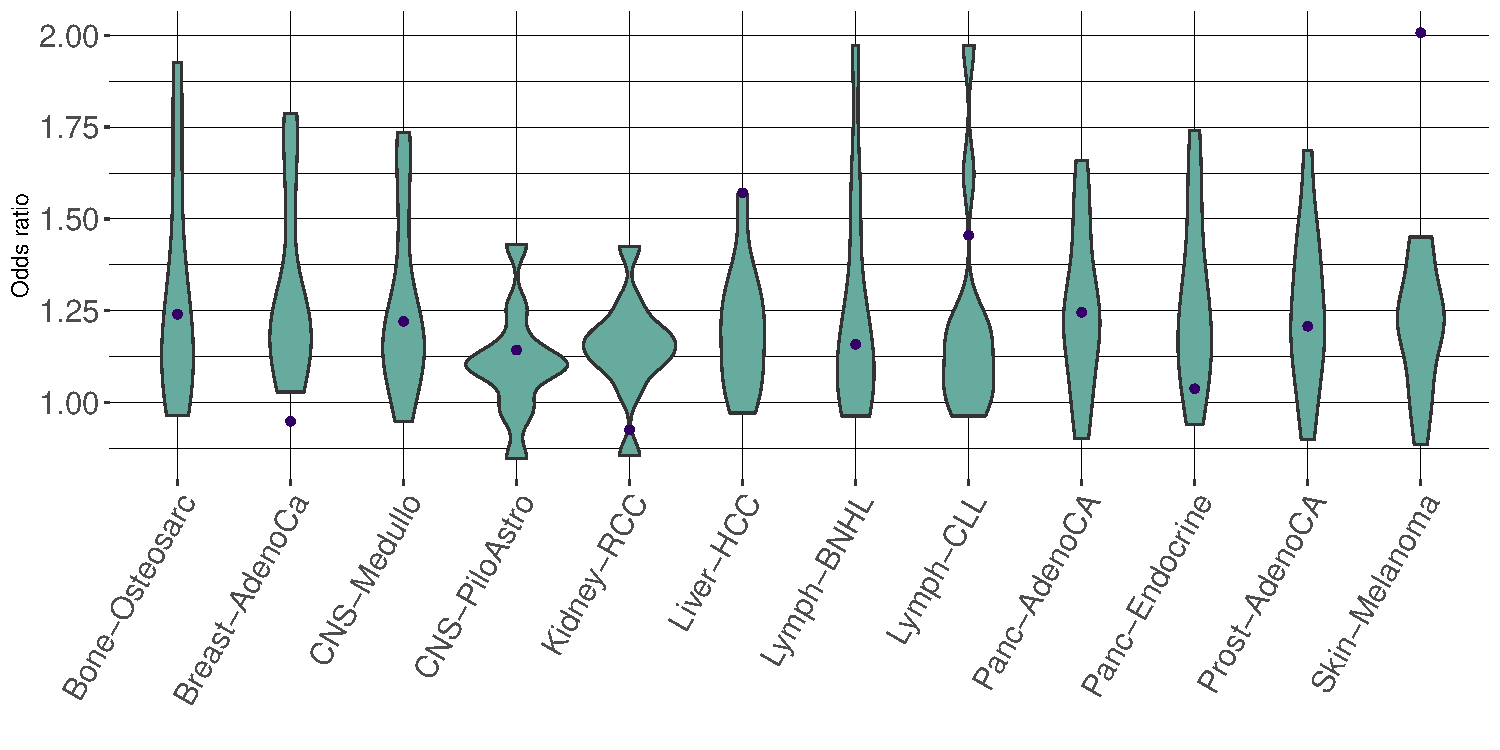
\includegraphics[scale=0.5]{graphics/mixed_or_violin.pdf}
    \caption{The impact of imbalanced DHS data on $OR$ is mild}
    \label{fig:mixed_or_violin}
    \end{subfigure} \\
    
    \vspace{0.3cm}
    \begin{subfigure}{\textwidth}
    \centering
    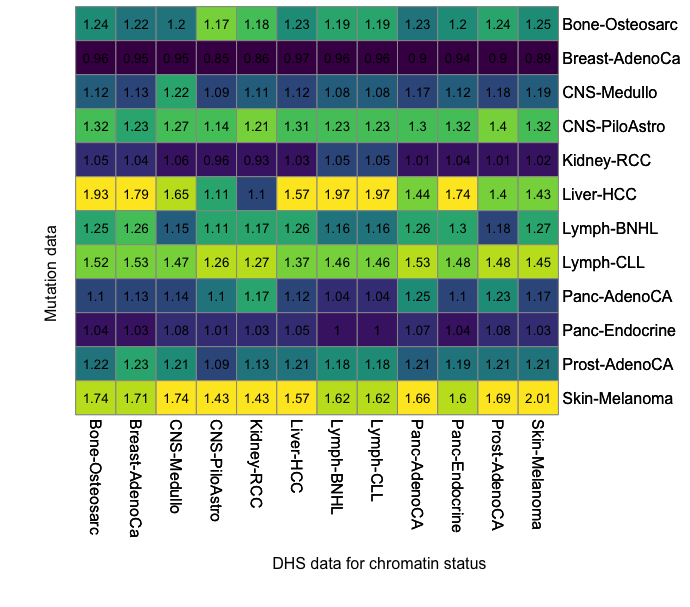
\includegraphics[scale=0.52]{graphics/mixed_or_heatmap.png}
    \caption{Chromatin structure is not discriminative of cancers}
    \label{fig:mixed_or_heatmap}
    \end{subfigure} 
\caption{}
    % \caption{\textbf{(a) The bias of mutations towards closed regions was not due to their large size compared to open regions but (b) this bias was unlikely the reason why GLE differs between cancers.} This figure shows an experiment where $OR$'s were calculated by cross-matching DHS data with mutation data of different cancers. In (a), the x-axis is the cancers whose DHS data was used, the y-axis is the distribution of $OR$ with mislabelled mutation data, with the purple dot indicating when mutation data of the correctly labelled cancer was used. In (b), the column labels are the cancers whose DHS data was used, the row labels are the cancers whose mutation data was used; each column is coloured by the rank of $OR$'s, brighter colours come from cancers whose mutation data produced the greater $OR$'s.}
    \label{fig:mixed_or}
\end{figure}

\section{GLE was significantly different between cancers}\label{gle:bootstrap}
Previously, we observed different patterns of GLE for different cancers by visualisation (Figure \ref{fig:mutation_density}). In this section, I investigated whether the difference is statistically significant and what data representations are optimal for GLE. For each pair of cancers, I used a bootstrap hypothesis test for whether their GLE's are significantly different. The bootstrap resulted in a p-value by comparing the observed distance to 1000 distances simulated under the null hypothesis that assumed there was no difference between cancer the pair (Methods \ref{methods:bootstrap}).

In addition to trialling the conventional bin representation \textit{v.s.} the proposed smooth representation, I also trialled two distance measures, Euclidean and Wasserstein, to see which representation/measure could best discriminate cancers. I trialled the Euclidean distance because it is the most widely used distance measures, and Wasserstein distance because it matches the nature of GLE data, which is the spatial distribution of mutations across the genome. The Euclidean distance is the point-wise difference between two vectors as it compares points that are strictly at the same coordinates, whereas the Wasserstein distance allows comparing points at different coordinates of the two vectors (illustrated in Methods Figure \ref{fig:wasserstein_demo}). I reported the raw p-values rather than recruiting multiple test correction because the true purpose of this section was to detect signals in the data and to compare the performance between representations. Therefore, it was not particularly meaningful to set a rigid significance threshold. From Figure \ref{fig:gle_bootstrap}, across both representations and distance measures, GLE was generally very different for all cancer pairs. The smooth representation was more likely to output smaller p-values, with only two pairs at p-values $>0.001$ for Wasserstein and no pairs for Euclidean distance. Note that the p-value matrices in Figure \ref{fig:gle_bootstrap} are symmetric. In addition, the most common cancer with p-value $>0.001$ was CNS-PiloAstro, which might be due to its small sample size, as in the case with the G-test and the $OR$. 

\begin{figure}[ht!]
    \begin{subfigure}{.5\textwidth}
    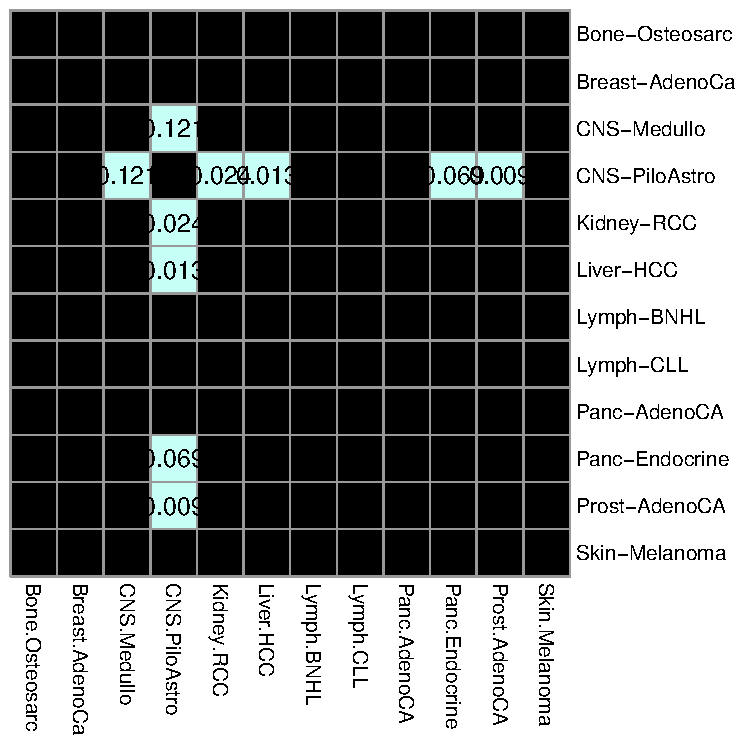
\includegraphics[scale=0.7]{graphics/bootstrap_bins_euclidean.pdf}
    \caption{Bins/Euclidean}
    \label{fig:bootstrap_bins_euclidean}
    \end{subfigure}
    ~
    \begin{subfigure}{.5\textwidth}
    
    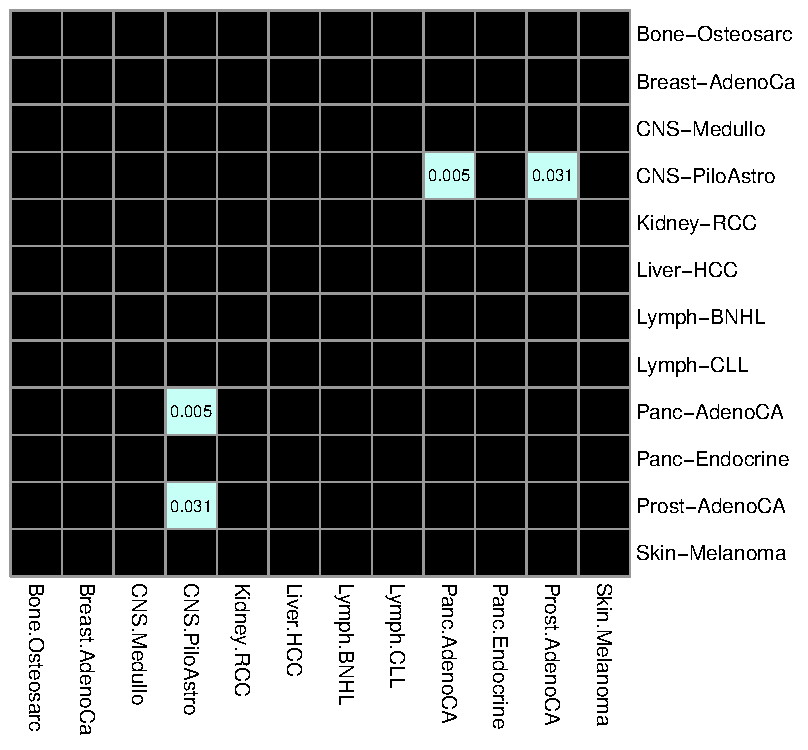
\includegraphics[scale=0.7]{graphics/bootstrap_bins_wasserstein.pdf}
    \caption{Bins/Wasserstein}
    \label{fig:bootstrap_bins_wasserstein}
    \end{subfigure} \\
    \vspace{0.5cm}
    
    \begin{subfigure}{.5\textwidth}
    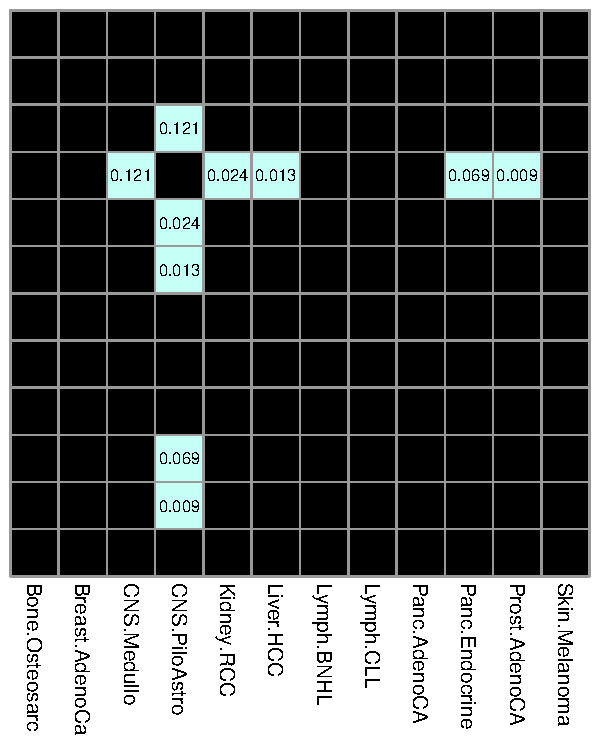
\includegraphics[width=\linewidth,height=0.7\textwidth]{graphics/bootstrap_smooth_euclidean.pdf}
    \caption{Smooth/Euclidean}
    \label{fig:bootstrap_smooth_euclidean}
    \end{subfigure}
    ~
    \begin{subfigure}{.5\textwidth}
    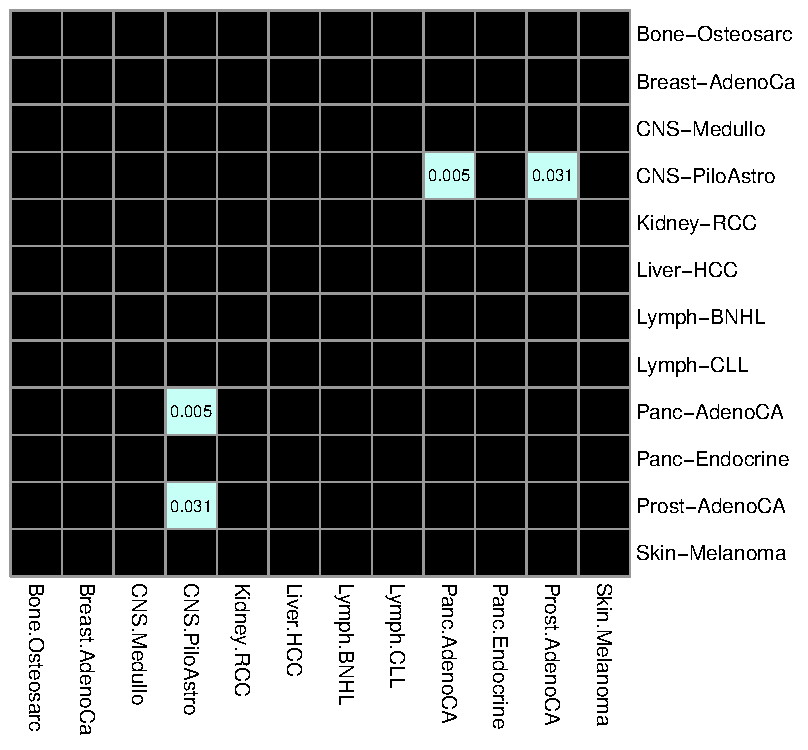
\includegraphics[width=\linewidth,height=0.7\textwidth]{graphics/bootstrap_smooth_wasserstein.pdf}
    \caption{Smooth/Wasserstein}
    \label{fig:smooth_wasserstein}
    \end{subfigure} \\
    
    \caption{\textbf{GLE was generally significantly different between cancers according to bootstrap hypothesis test using (a) Bin/Euclidean, (b) Bin/Wasserstein, (c) Smooth/Euclidean, (d) Smooth/Wasserstein.} No multiple test correction was applied. All estimated p-values were $<0.001$ unless otherwise specified.}
    \label{fig:bootstrap}
\end{figure}

\section{Chapter summary}
Overall, the analysis of GLE shows that GLE is an important characteristic of a cancer mutation profile. In particular, GLE was influenced by chromatin structure and it differed between cancers, but the former was unlikely to be causal of the latter. In section \ref{gle:chromatin}, I showed that mutations tended to occur in closed chromatin regions compared to open chromatin regions by visualisation and by formal statistical techniques. These techniques include the G-test of independence, which showed that the distribution of mutations were significantly different between open and closed regions (subsection \ref{gle:g}) and the $OR$ statistic, which showed that mutations were biased towards closed chromatin regions (subsection \ref{gle:or}). The mislabelling experiment in subsection \ref{gle:mixed_or} shows that $OR$ is an appropriate measure of mutations bias in that it was not impacted by the imbalanced sizes between open and closed chromatin regions. However, subsection \ref{gle:mixed_or} also showed that chromatin structure was unlikely to determine whether GLE differed between cancers or not. In section \ref{gle:bootstrap}, using hypothesis tests by bootstrapping, GLE was shown to significantly differ between cancers, irrespective of the driving mechanisms. More importantly, smoothing GLE was demonstrated to be better at extracting information from mutation location than binning for both Euclidean and Wasserstein distances because it produced more significant p-values for differentiating cancers.
